%%% LaTeX Template: Two column article
%%%
%%% Source: http://www.howtotex.com/
%%% Feel free to distribute this template, but please keep to referal to http://www.howtotex.com/ here.
%%% Date: February 2011

%%% Preamble
\documentclass[	DIV=calc,%
							paper=a4,%
							fontsize=12pt,%
							onecolumn]{scrartcl}	 					% KOMA-article class

\usepackage{lipsum}													% Package to create dummy text
\usepackage[brazil]{babel}										% English language/hyphenation
\usepackage[protrusion=true,expansion=true]{microtype}				% Better typography
\usepackage{amsmath,amsfonts,amsthm}					% Math packages
\usepackage[pdftex]{graphicx}									% Enable pdflatex
\usepackage[svgnames]{xcolor}									% Enabling colors by their 'svgnames'
\usepackage[hang, small,labelfont=bf,up,textfont=it,up]{caption}	% Custom captions under/above floats
\usepackage{epstopdf}												% Converts .eps to .pdf
\usepackage{subfig}													% Subfigures
\usepackage{booktabs}												% Nicer tables
\usepackage{fix-cm}													% Custom fontsizes
\usepackage[utf8]{inputenc}
\usepackage[top=2.5cm, bottom=2.5cm, left=2.5cm, right=2.5cm]{geometry}
\usepackage[ddmmyyyy]{datetime}
\addto\captionsenglish{%
	\renewcommand\tablename{Tabela}
	\renewcommand\figurename{Figura}
} 
 

 
%%% Custom sectioning (sectsty package)
\usepackage{sectsty}													% Custom sectioning (see below)
\allsectionsfont{%															% Change font of al section commands
	\usefont{OT1}{phv}{b}{n}%										% bch-b-n: CharterBT-Bold font
	}

\sectionfont{%																% Change font of \section command
	\usefont{OT1}{phv}{b}{n}%										% bch-b-n: CharterBT-Bold font
	}



%%% Headers and footers
\usepackage{fancyhdr}												% Needed to define custom headers/footers
	\pagestyle{fancy}														% Enabling the custom headers/footers
\usepackage{lastpage}	

% Header (empty)
\lhead{}
\chead{}
\rhead{}
% Footer (you may change this to your own needs)

%% ====================================
%% ====================================
%% mude o rodape  do projeto
%% ====================================
%% ====================================

\lfoot{\footnotesize \texttt{cabeamento estruturado} \textbullet ~Modelo de projeto}


\cfoot{}
\rfoot{\footnotesize página \thepage\ de \pageref{LastPage}}	% "Page 1 of 2"
\renewcommand{\headrulewidth}{0.0pt}
\renewcommand{\footrulewidth}{0.4pt}



%%% Creating an initial of the very first character of the content
\usepackage{lettrine}
\newcommand{\initial}[1]{%
     \lettrine[lines=3,lhang=0.3,nindent=0em]{
     				\color{DarkGoldenrod}
     				{\textsf{#1}}}{}}



%%% Title, author and date metadata
\usepackage{titling}															% For custom titles

\newcommand{\HorRule}{\color{DarkGoldenrod}%			% Creating a horizontal rule
									  	\rule{\linewidth}{1pt}%
										}

\pretitle{\vspace{-30pt} \begin{flushleft} \HorRule 
				\fontsize{50}{50} \usefont{OT1}{phv}{b}{n} \color{DarkRed} \selectfont 
				}

%% ====================================
%% ====================================
%% mude o titulo  do projeto
%% ====================================
%% ====================================

\title{Projeto de cabeamento estruturado - Empresa FourBR}					% Title of your article goes here

%% ====================================



\posttitle{\par\end{flushleft}\vskip 0.5em}

\preauthor{\begin{flushleft}
					\large \lineskip 0.5em \usefont{OT1}{phv}{b}{sl} \color{DarkRed}}
\author{Arthur Garcia Vianna }  	% Author name goes here


\postauthor{\footnotesize \usefont{OT1}{phv}{m}{sl} \color{Black} 
					\\Universidade Tecnológica Federal do Paraná - Câmpus Cornélio Procópio 								% Institution of author
					\par\end{flushleft}\HorRule}

\date{}																				% No date




%%% Begin document
\begin{document}
\maketitle
\thispagestyle{fancy} 	
\thispagestyle{empty}		% Enabling the custom headers/footers for the first page 
% The first character should be within \initial{}




%% ====================================
%% ====================================
%% mude o resumo  do projeto
%% ====================================
%% ====================================
\initial{N}\textbf{este projeto será detalhado todo o processo de cabeamento estruturado que será desenvolvido para a empresa FourBR, uma empresa nacional de marketing digital de pequeno porte, que atualmente possui sua rede de computadores executada de maneira extremamente obsoleta e não-funcional. Através deste projeto todos os pontos de rede serão conectados de maneira eficiente garantindo assim o compartilhamento eficaz de dados com segurança.}

%% ====================================
\begin{figure}
	\centering
	
\includegraphics{utfpr}
\end{figure}

\vspace{3cm}
\centerline{\textit{\textbf{\today}}}

\clearpage
    \renewcommand*\listfigurename{Lista de figuras}
\listoffigures






\clearpage
\renewcommand{\contentsname}{Sumário}
\tableofcontents
\clearpage

%% ====================================
%% ====================================
%% Inicio do texto
%% ====================================
%% ====================================
\section{Introdução}
A empresa FourBR dispõe no momento de 15 notebooks, em um escritório de 60 metros quadrados, conectados entre si através de um hub que é ligado diretamente em um roteador ADSL.
Não existe acesso a internet através de wireless e a colisão de dados é enorme devido à conexão realizada através de um hub, que por si só possui apenas um domínio de colisão e funciona no modelo half-duplex.
Serão instalados um roteador, um switch e um firewall de boa qualidade para garantir um fluxo de dados eficiente na rede, além de toda a parte de cabeamento estruturado e certificação dos cabos e pontos de rede.
Serão também projetados planos de contenção em caso de falhas e manutenções periódicas.
\subsection{Benefícios}
Alguns dos benefícios deste projeto seriam a comunicação fluida entre os usuários da rede interna e externa, extermínio de colisão de dados na rede, acesso cabeado e sem fio a rede, além da estabilidade e segurança da rede, garantindo assim que o foco principal da empresa, o marketing digital, seja realizado de maneira eficiente e sem problemas.

\subsection{Organizações Envolvidas}
A empresa ConsultPW cuidará de toda a parte do projeto, desde o orçamento até a implementação dos dispositivos e da arquitetura. A empresa de TI conta com 3 equipes sendo elas:

\begin{itemize}
\item Financeira
\item Projeto
\item Técnica
\end{itemize}


\section{Estado atual}
Rede extremamente instável e com muito travamento devido principalmente aos seguintes fatores:

\begin{itemize}
	\item Utilização de hub
	\item Roteador simples de uso doméstico
	\item Cabeamento mal realizado, com falhas e torções
	\item Cabos CAT5E
	\item Inexistência de racks ou sala de servidores e dispositivos
	\item Model ADSL de baixo desempenho
	\item Hub de 16 portas
	
\end{itemize}

\section{Requisitos}
Será necessário que o ambiente seja desocupado pelo prazo inicial de 4 semanas para que todo o projeto seja desenvolvido, desde a passagem de cabos pelas canaletas até a montagem da topologia física e lógica da rede.

\section{Usuários e Aplicativos}
Atualmente a empresa conta com 15 funcionários/usuários que utilizam os end-points e que precisam ter acesso aos recursos da rede de maneira ininterrupta. A empresa tem um plano de crescimento a longo prazo e portanto o projeto abordará esse requisito no momento de definir, planejar e implementar o plano de escalabilidade da rede.
 

\subsection{Usuários}
São 15 usuários que possuem conhecimento em informática de nível baixo ao médio e que utilizam quase que diariamente os mesmos softwares que se enquadram no padrão da empresa, além de softwares mundialmente utilizados para edição e leitura de textos, planilhas e apresentações de slides.
Destes 15 usuários existem:

\begin{itemize}
	\item 2 gerentes
	\item 10 funcionários efetivos
	\item 3 estagiários

	
\end{itemize}

\subsection{Aplicativos}
\begin{itemize}
	\item Microsoft Office 2016
	\item Adobe Reader
	\item Adobe Photoshop CS6
	\item WinRAR
	\item Google Chrome
	\item One Drive
	\item Aplicativos standard da empresa
	
	
\end{itemize}


\section{Estrutura predial existente}

Atualmente o escritório conta com 60 metros quadrados, sendo estes divididos em 7 ambientes diferentes. Alguns desses ambientes contém funcionários que necessitam do acesso à rede para executar suas funções diárias. A distância entre os pontos de rede vai variar de acordo com o ambiente, sendo que a planta do escritório irá descrever com maiores detalhes o planejamento do processo.

\section{Planta Lógica - Elementos estruturados}



\subsection{Topologia}

Serão utilizados 20 metros de cabo UTP categoria 6 (Cat6) para realizar toda a intregração dos end-points e dos dispositivos de rede mostrados na Figura 1. Os cabos serão passados através de canaletas implementadas diretamente na parede seguindo o padrão de cabeamento horizontal. Os dispostivos de rede, sendo eles, um pacth panel, um switch de 24 portas, um roteador empresarial e um firewall ficam na sala de rack. Um access point de alto alcance ficará localizado exatamento no meio do escritório entre a sala de funcionários e a sala do gerente 2. Serão instaladas também 15 tomadas com entrada RJ-45 fêmea para que os usuários possam se conectar a rede ethernet. Todos os cabos serão crimpados utilizando a norma T-568A.

\begin{figure}[h]
	\centering
	\flushright
	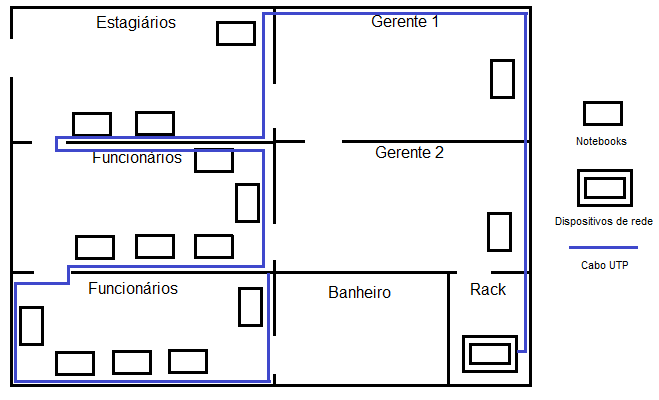
\includegraphics[scale=0.6]{planta}
	\caption{Planta do projeto a ser implementado.}
	\label{fplanta}
\end{figure}

\begin{figure}[h]
	\centering
	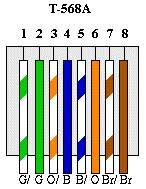
\includegraphics[scale=0.6]{index}
	\caption{Padrão de crimpagem dos cabos UTP.}
	\label{T658A}
\end{figure}

\subsection{Encaminhamento}
Os cabos serão encaminhado através de 25 metros de eletrodutos fixados nas paredes do escritório.

\subsection{Memorial descritivo}

\begin{figure}[h]
	\centering
	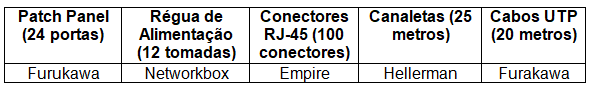
\includegraphics[scale=0.6]{tab}
	\caption{Tabela de passivos de rede.}
	\label{tab}
\end{figure}

\subsection{Identificação dos cabos}
Todos os cabos serão rotulados através de fitas adesivas de cores diferentes que indicarão o tipo de dispositivo que está sendo conectado e o número das conexões nas portas do switch.

\section{Implantação}
\begin{figure}[h]
	\centering
	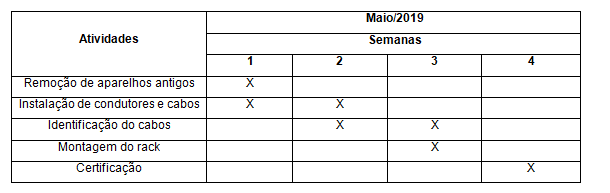
\includegraphics[scale=0.6]{crono}
	\caption{Cronograma do projeto.}
	\label{crono}
\end{figure} 

\section{Plano de certificação}
A certificação será realizada em toda a rede através do equipamento de certificação Lantek III. Todos os patch cords e patch panels e demais dispostivos da rede. A certificação será realizada no próprio escritório na última semana de projeto, sendo este o último passo a ser realizado. Todo o processo será documentado e entregue aos contratantes por meio de relatórios detalhados da certificação.  

\section{Plano de manutenção}

Serão realizadas revisões periódicas a 1 vez por ano, sempre no mês de maio, conforme consta em contrato. 

\subsection{Plano de expansão}
A empresa pretende aumentar seus pontos de rede no futuro de acordo com o seu crescimento, porém, no momento não existem planos de expansão a curto prazo. Mesmo assim, existem 9 portas não utilizadas no switch, exigindo apenas a instalação de mais tomadas com conectores RJ-45 fêmea.  

\section{Risco}
Os riscos são relativamente pequenos levando em consideração que toda a rede será certificada com um nível muito grande de detalhamento, porém em caso de qualquer problema a empresa estará disponível para o mais rápido atendimento. 

\section{Orçamento}
A mão de obra da empresa contratada será discutida com os responsáveis pela FourBR.
\begin{figure}[h]
	\centering
	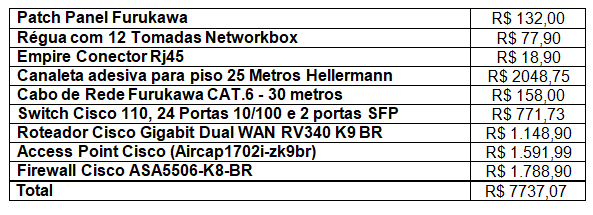
\includegraphics[scale=0.6]{orac}
	\caption{Orçamento do projeto.}
	\label{orac}
\end{figure} 

\section{Recomendações}
Os usuários serão devidamente treinados para manusear seus equipamentos da maneira correta, mantendo assim a funcionalidade da rede. Instalações, manutenções ou reparos na rede são expressamente proibidos quando não realizados por funcionários qualificados de nossa empresa.




%% ***********************************************************************
%% === remover daqui =====================================================
%% ***********************************************************************




%% ***********************************************************************
%% === ate aqui    =====  ================================================
%% ***********************************************************************

\end{document}